\chapter{Adaptive Immunity and Vaccination}\label{ch:b3:adaptive-immunity}

In 1796 a country doctor scratched pus from a milkmaid's cowpox sore
into the arm of a boy, and six weeks later inoculated him with smallpox;
the boy did not fall ill. In 1980 the World Health Organization
declared smallpox --- which had killed three hundred million people in
the twentieth century --- eradicated from the Earth, by that method. The
system that Jenner had recruited, without knowing it existed, can
recognise any molecule it has never met, choose among a hundred billion
different receptors the few that fit, multiply the cells that carry
them a millionfold in a week, improve their fit by mutation and
selection while it does so, and remember the result for a lifetime; it
also learns not to attack the body that made it, and its failures to
learn that are the autoimmune diseases. This chapter treats the
\omterm{def:b3:adaptive-immunity:lymphocytes}{lymphocytes} and how they make their receptors, how a response is
mounted and remembered, how \omterm{def:b3:adaptive-immunity:tolerance}{tolerance} is enforced and lost, and the
arithmetic by which vaccinating enough people protects those who are
not.

\section{Lymphocytes and clonal selection}

\begin{definition}[Lymphocytes and their receptors]\label{def:b3:adaptive-immunity:lymphocytes}
\index{lymphocyte}\index{B cell}\index{T cell}\index{antigen}\index{clonal selection}\index{lymph node}
\emph{Adaptive immunity} is carried by \emph{lymphocytes}: \emph{B cells},
which mature in the bone marrow and whose antigen receptor is a
membrane-bound \emph{\omterm{def:b3:adaptive-immunity:antibody}{antibody}} that they later secrete; and \emph{T
cells}, which mature in the \omterm{def:b3:adaptive-immunity:tolerance}{thymus} and whose receptor recognises
peptide fragments displayed on the surface of other cells. An
\emph{antigen} is whatever a receptor binds; the part actually
contacted is an \emph{epitope}. The founding fact is \emph{clonal
selection} (Burnet, 1957): each lymphocyte carries receptors of one
specificity only, fixed before it meets any antigen; the body holds a
repertoire of some $10^{11}$ such cells; an antigen selects the few
whose receptors fit and drives them to divide into a clone of effector
and \omterm{def:b3:adaptive-immunity:response}{memory cells}; and lymphocytes whose receptors fit the body's own
molecules are deleted or silenced while they mature. The cells
circulate continuously between the blood and the \emph{lymph nodes},
spleen and mucosal lymphoid tissue, where antigen carried by \omterm{def:b3:innate-immunity:innate}{dendritic
cells} (\cref{ch:b3:innate-immunity}) is displayed, so that the rare
matching cell --- one in a hundred thousand for a given epitope ---
finds it within a day or two.
\end{definition}

\begin{proof}[Evidence]
Nossal and Lederberg (1958) placed single \omterm{def:b3:adaptive-immunity:lymphocytes}{lymphocytes} from immunised
rats in microdroplets and tested the \omterm{def:b3:adaptive-immunity:antibody}{antibody} each secreted: every
cell made \omterm{def:b3:adaptive-immunity:antibody}{antibody} against one of the two \omterm{def:b3:adaptive-immunity:lymphocytes}{antigens}, never both. Burnet
had predicted it the year before. Tonegawa (1976) compared the DNA of
an \omterm{def:b3:adaptive-immunity:antibody}{antibody} gene in embryonic cells and in an antibody-secreting
\omterm{def:b3:cancer-biology:hallmarks}{tumour}: in the embryo the variable and constant parts lay far apart, in
the \omterm{def:b3:cancer-biology:hallmarks}{tumour} they were joined --- the gene had been cut and spliced in
the somatic cell, the first demonstration of a genome rearranged on
purpose.
\end{proof}

\section{Making a hundred billion receptors}

\begin{definition}[Antibody structure and V(D)J recombination]\label{def:b3:adaptive-immunity:antibody}
\index{antibody}\index{immunoglobulin}\index{V(D)J recombination}\index{RAG}\index{junctional diversity}\index{class switching}
An \emph{antibody} (immunoglobulin) is two identical heavy chains and
two identical light chains, each with a \emph{variable} domain at its
end and \emph{constant} domains behind; the two arms each bind an
epitope through three hypervariable loops of the heavy and three of
the light variable domain, and the stem (Fc) is what phagocytes,
\omterm{def:b3:innate-immunity:complement}{complement} and mast cells recognise. Five classes differ in their
heavy-chain constant region: IgM, the first made, a pentamer that
activates \omterm{def:b3:innate-immunity:complement}{complement} well; IgG, the workhorse of blood and tissues,
which crosses the placenta; IgA, a dimer secreted across mucosal
surfaces into gut, airways and milk; IgE, bound by mast cells, against
worms --- and the cause of allergy; IgD. The variable domains are not
encoded as such. The heavy-chain locus holds about $40$ functional
\emph{V} segments, $25$ \emph{D} and $6$ \emph{J}; a developing B~cell
chooses one of each and joins them by \emph{V(D)J recombination}: the
enzymes RAG1 and RAG2 cut at recombination signal sequences flanking
the segments, and the ends are joined by the non-homologous end-joining
machinery of \cref{ch:b3:dna-repair}, with nucleotides trimmed and
added at random (by the enzyme TdT) at each junction --- \emph{junctional
diversity}, which falls exactly in the third hypervariable loop. The
light chains do the same with V and J. After the response begins the
same variable domain is joined to a different constant region by a
second rearrangement, \emph{class switching}, changing the antibody's
function but not its specificity.
\end{definition}

\begin{theorem}[The size of the repertoire]\label{thm:b3:adaptive-immunity:repertoire}
\index{repertoire!combinatorial}
With $V_{H} = 40$, $D = 25$, $J_{H} = 6$ heavy segments, and light chains
from two loci with $(V_{\kappa}, J_{\kappa}) = (40, 5)$ and
$(V_{\lambda}, J_{\lambda}) = (30, 4)$, the number of distinct
heavy--light combinations obtainable by segment choice alone is
\[
(40\times 25\times 6)\times(40\times 5 + 30\times 4) = 6000\times 320
= 1.9\times 10^{6}.
\]
\omterm{def:b3:adaptive-immunity:antibody}{Junctional diversity} at the two heavy junctions and one light junction
multiplies this by a factor of order $10^{4}$--$10^{5}$, giving a
potential repertoire above $10^{10}$ from fewer than $200$ gene
segments --- more than the number of B~cells in a body, so that the
actual repertoire is a sample of the possible one. \omterm{def:b3:adaptive-immunity:germinal-centre}{Somatic
hypermutation} during the response (below) then generates variants of
each selected receptor.
\end{theorem}
\begin{proof}
Each heavy chain is one V, one D and one J; each light chain one V and
one J from either locus; any heavy pairs with any light, so the counts
multiply (multiplication principle), and the two light loci add. The
junctional factor is the number of distinct sequences the random
trimming and addition can produce at a junction --- a few dozen per
junction at least --- raised to the number of junctions; its exact value
is not defined, but three junctions each with $30$--$50$ outcomes give
$3\times 10^{4}$ to $10^{5}$. The count for T~cell receptors, with two
chains rearranged in the same way and a larger junctional contribution,
is of the same order.
\end{proof}

\begin{omfigure}
\begin{tikzpicture}[every node/.style={font=\scriptsize}, >=stealth]
  % antibody Y
  \begin{scope}[xshift=0cm]
    % heavy chains
    \draw[very thick, omDef] (0,0) -- (0,1.6) -- (-1.3,3.0); \draw[very thick, omDef] (0.35,0) -- (0.35,1.6) -- (1.65,3.0);
    % light chains
    \draw[very thick, omProp] (-0.45,1.55) -- (-1.75,2.95); \draw[very thick, omProp] (0.8,1.55) -- (2.1,2.95);
    \fill[omThm] (-1.55,3.0) circle (0.12); \fill[omThm] (1.9,3.0) circle (0.12);
    \node[above, align=center] at (-1.5,3.15) {variable domains:\\antigen-binding site}; 
    \node[right, align=left] at (0.55,0.5) {Fc stem (constant):\\class decides function};
    \node[left, omProp] at (-0.7,2.1) {light}; \node[right, omDef] at (0.4,1.3) {heavy};
    \draw[omDef] (0.05,1.1) -- (0.3,1.1); \draw[omDef] (0.05,0.7) -- (0.3,0.7);
  \end{scope}
  % V(D)J locus
  \begin{scope}[xshift=4.2cm, yshift=2.4cm, xscale=0.86]
    \draw[very thick, gray] (0,0) -- (8.2,0);
    \foreach \x in {0.2,0.6,1.0,1.4} \draw[thick, fill=omDef!40] (\x,-0.15) rectangle (\x+0.3,0.15);
    \node[above] at (0.95,0.2) {V segments ($\sim 40$)}; \node[font=\tiny] at (1.95,0) {$\cdots$};
    \foreach \x in {2.5,2.8,3.1} \draw[thick, fill=omProp!50] (\x,-0.15) rectangle (\x+0.2,0.15);
    \node[above] at (2.9,0.2) {D ($25$)};
    \foreach \x in {3.8,4.1,4.4} \draw[thick, fill=omMeth!50] (\x,-0.15) rectangle (\x+0.2,0.15);
    \node[above] at (4.2,0.2) {J ($6$)};
    \foreach \x/\lab in {5.3/\mu,6.0/\delta,6.7/\gamma,7.4/\alpha} { \draw[thick, fill=gray!30] (\x,-0.15) rectangle (\x+0.5,0.15); \node[above] at (\x+0.25,0.2) {C$_{\lab}$}; }
    \draw[->, thick] (4.1,-0.4) -- (4.1,-1.1) node[midway, right, align=left, font=\tiny] {RAG cuts at the signal sequences; one V, one D,\\one J are joined, TdT adds random nucleotides};
    % rearranged
    \draw[very thick, gray] (0,-1.5) -- (3.3,-1.5);
    \draw[thick, fill=omDef!40] (1.0,-1.65) rectangle (1.3,-1.35); \fill[omThm] (1.3,-1.65) rectangle (1.4,-1.35);
    \draw[thick, fill=omProp!50] (1.4,-1.65) rectangle (1.6,-1.35); \fill[omThm] (1.6,-1.65) rectangle (1.7,-1.35);
    \draw[thick, fill=omMeth!50] (1.7,-1.65) rectangle (1.9,-1.35);
    \draw[thick, fill=gray!30] (2.6,-1.65) rectangle (3.1,-1.35); \node[above] at (2.85,-1.3) {C$_{\mu}$};
    \node[below, align=center] at (1.45,-1.7) {VDJ joined: the variable domain,\\red: junctional nucleotides};
    \node[right, align=left, font=\tiny] at (3.4,-2.0) {spliced to C$_{\mu}$: an IgM heavy chain;\\class switching later joins the same\\VDJ to C$_{\gamma}$ or C$_{\alpha}$};
  \end{scope}
\end{tikzpicture}

{\small Left: an \omterm{def:b3:adaptive-immunity:antibody}{antibody} --- two heavy and two light chains, the
variable domains at the tips forming two binding sites, the constant
stem read by the rest of the immune system. Right: the heavy-chain
locus before and after \omterm{def:b3:adaptive-immunity:antibody}{V(D)J recombination}, which picks one segment of
each kind and adds random nucleotides at the joins.}
\end{omfigure}

\begin{definition}[T~cell receptors and MHC]\label{def:b3:adaptive-immunity:mhc}
\index{T cell receptor}\index{major histocompatibility complex}\index{antigen presentation}\index{MHC restriction}\index{HLA}
The \emph{T~cell receptor} is a two-chain molecule built by the same
recombination, never secreted, and it does not bind \omterm{def:b3:adaptive-immunity:lymphocytes}{antigen} free in
solution: it recognises a short peptide held in the groove of a
\emph{major histocompatibility complex} (MHC) molecule on another
cell's surface. \emph{MHC class~I}, on every nucleated cell, displays
peptides of eight to ten residues cut by the proteasome from the
cell's own cytosolic proteins --- a sample of what the cell is making,
including any \omterm{def:b3:virology:virus}{virus} --- to \emph{CD8} T~cells, which kill the cell if
the peptide is foreign. \emph{MHC class~II}, on \omterm{def:b3:innate-immunity:innate}{dendritic cells},
\omterm{def:b3:innate-immunity:innate}{macrophages} and B~cells, displays peptides of thirteen to twenty-five
residues from proteins the cell has taken up and digested in
\omterm{def:b3:membrane-traffic:endocytosis}{endosomes}, to \emph{CD4} T~cells, which respond by helping. A T~cell
is \emph{restricted}: it recognises its peptide only on the MHC allele
it was selected on. The MHC genes (\emph{HLA} in humans) are the most
polymorphic in the genome, with thousands of alleles each differing in
the groove, so that each person displays a different sample of each
protein's peptides and no pathogen can escape presentation in everyone
--- and so that a transplanted organ from an unmatched donor is
recognised as foreign by a large fraction of the recipient's T~cells.
\end{definition}

\begin{proof}[Evidence]
Zinkernagel and Doherty (1974) infected mice of two inbred strains with
a \omterm{def:b3:virology:virus}{virus} and tested their cytotoxic T~cells on infected target cells:
the T~cells killed infected cells of their own strain but not of the
other, although the \omterm{def:b3:virology:virus}{virus} was the same. The T~cell saw the \omterm{def:b3:virology:virus}{virus} only
together with a self MHC molecule --- \emph{\omterm{def:b3:adaptive-immunity:mhc}{MHC restriction}} --- which
was later explained when the crystal structure of an MHC molecule
(Bjorkman, 1987) showed a groove with a peptide in it, and the T~cell
receptor was shown to bind the two together.
\end{proof}

\begin{omfigure}
\begin{tikzpicture}[every node/.style={font=\scriptsize}, >=stealth]
  % class I pathway
  \begin{scope}
    \draw[thick, omDef, fill=omDef!8] (0,0) rectangle (6.2,3.6); \node[anchor=north west] at (0.05,3.55) {any nucleated cell};
    \node[draw, rounded corners, fill=omThm!20, font=\tiny, align=center] (v) at (1.4,2.6) {viral or self protein\\in the cytosol};
    \node[draw, rounded corners, fill=gray!20, font=\tiny, align=center] (p) at (1.4,1.5) {proteasome:\\peptides of 8--10};
    \node[draw, rounded corners, fill=omDef!25, font=\tiny, align=center] (er) at (4.6,1.5) {ER: loaded on\\MHC class I};
    \draw[->, thick] (v) -- (p); \draw[->, thick] (p) -- node[midway, above, font=\tiny] {TAP} (er);
    \draw[->, thick] (er) -- (4.6,3.55);
    \draw[thick, fill=omDef!40] (4.4,3.6) rectangle (4.8,4.1); \fill[omThm] (4.6,4.2) circle (0.09);
    \node[above, align=center] at (4.6,4.35) {peptide--MHC I\\seen by CD8 T cells: kill};
  \end{scope}
  % class II pathway
  \begin{scope}[xshift=7.2cm]
    \draw[thick, omProp, fill=omProp!8] (0,0) rectangle (6.2,3.6); \node[anchor=north west] at (0.05,3.55) {dendritic cell, macrophage, B cell};
    \node[draw, rounded corners, fill=omThm!20, font=\tiny, align=center] (ex) at (1.4,2.6) {protein taken up\\into an endosome};
    \node[draw, rounded corners, fill=gray!20, font=\tiny, align=center] (dig) at (1.4,1.5) {digested:\\peptides of 13--25};
    \node[draw, rounded corners, fill=omProp!30, font=\tiny, align=center] (m2) at (4.6,1.5) {MHC class II\\loaded here};
    \draw[->, thick] (ex) -- (dig); \draw[->, thick] (dig) -- (m2);
    \draw[->, thick] (m2) -- (4.6,3.55);
    \draw[thick, fill=omProp!50] (4.4,3.6) rectangle (4.8,4.1); \fill[omThm] (4.6,4.2) circle (0.09);
    \node[above, align=center] at (4.6,4.35) {peptide--MHC II\\seen by CD4 T cells: help};
  \end{scope}
\end{tikzpicture}

{\small The two presentation pathways. Class~I shows CD8 T~cells what
a cell is making inside itself; class~II shows CD4 T~cells what an
antigen-presenting cell has eaten. A cytotoxic response is aimed at
the first, a helper response at the second.}
\end{omfigure}

\section{The response}

\begin{definition}[Activation, help and killing]\label{def:b3:adaptive-immunity:response}
\index{helper T cell}\index{cytotoxic T cell}\index{costimulation}\index{regulatory T cell}\index{plasma cell}\index{memory cell}
A naive T~cell is activated when its receptor binds peptide--MHC on a
\omterm{def:b3:innate-immunity:innate}{dendritic cell} that also provides costimulation (\cref{ch:b3:innate-immunity});
it then divides every six to eight hours for a week and differentiates.
\emph{CD4 helper} T~cells differentiate, according to the \omterm{def:b3:innate-immunity:innate}{dendritic
cell}'s \omterm{def:b3:innate-immunity:inflammation}{cytokines}, into subsets: Th1, which activate \omterm{def:b3:innate-immunity:innate}{macrophages} to kill
what they have eaten (tuberculosis); Th2, which drive IgE and
eosinophils against worms; Th17, which recruit \omterm{def:b3:innate-immunity:innate}{neutrophils} against
extracellular bacteria and fungi; follicular helpers, which help
B~cells; and \emph{regulatory} T~cells, which suppress. \emph{CD8
cytotoxic} T~cells kill cells displaying their peptide on class~I, by
perforin and granzymes and by the Fas ligand, triggering \omterm{def:b3:cell-cycle-apoptosis:apoptosis}{apoptosis}
(\cref{ch:b3:cell-cycle-apoptosis}) --- the defence against viruses and
\omterm{def:b3:cancer-biology:hallmarks}{tumours}. A B~cell is activated by \omterm{def:b3:adaptive-immunity:lymphocytes}{antigen} binding its receptor plus
help from a follicular helper T~cell that recognises peptides of the
same \omterm{def:b3:adaptive-immunity:lymphocytes}{antigen} on the B~cell's class~II; it then becomes a \emph{plasma
cell} secreting thousands of antibodies a second, for days (short-lived,
in the node) or years (long-lived, in the marrow), or enters a \omterm{def:b3:adaptive-immunity:germinal-centre}{germinal
centre}. \emph{Memory} B and T~cells --- long-lived, more numerous than
the naive precursors and quicker to respond --- are the residue of every
response and the basis of vaccination.
\end{definition}

\begin{definition}[The germinal centre]\label{def:b3:adaptive-immunity:germinal-centre}
\index{germinal centre}\index{somatic hypermutation}\index{affinity maturation}
In a \emph{germinal centre}, a structure that forms in a \omterm{def:b3:adaptive-immunity:lymphocytes}{lymph node}
about a week into a response, activated B~cells run an evolutionary
algorithm. In its dark zone they divide every six hours and their
\omterm{def:b3:adaptive-immunity:antibody}{antibody} variable genes are mutated by the enzyme AID at about one
change per thousand base pairs per division --- \emph{somatic
hypermutation}, a million times the genomic rate, aimed at one
kilobase. In the light zone each cell tests its new receptor against
\omterm{def:b3:adaptive-immunity:lymphocytes}{antigen} held on follicular \omterm{def:b3:innate-immunity:innate}{dendritic cells} and competes for the help of
T~cells: cells that bind better take up more \omterm{def:b3:adaptive-immunity:lymphocytes}{antigen}, present more,
receive more help and return to the dark zone to divide again; cells
that bind worse, or have lost binding, die by \omterm{def:b3:cell-cycle-apoptosis:apoptosis}{apoptosis}. Over two to
three weeks of cycles the affinity of the surviving antibodies rises a
hundred- to a thousandfold --- \emph{affinity maturation} --- and the
winners leave as \omterm{def:b3:adaptive-immunity:response}{plasma cells} and \omterm{def:b3:adaptive-immunity:response}{memory cells}, having also switched
class. The secondary response is faster, larger and made of better
\omterm{def:b3:adaptive-immunity:antibody}{antibody} because it starts from this selected, expanded, switched
population.
\end{definition}

\begin{omfigure}
\begin{tikzpicture}[every node/.style={font=\scriptsize}, >=stealth]
  \draw[thick, omDef, fill=omDef!12] (0,0) ellipse (2.7 and 1.7); \node[above, omDef!70!black] at (0,1.75) {dark zone};
  \draw[thick, omMeth!70!black, fill=omMeth!12] (6.2,0) ellipse (2.7 and 1.7); \node[above, omMeth!60!black] at (6.2,1.75) {light zone};
  \node[align=center] at (0,0.3) {B cells divide every \qty{6}{h};\\AID mutates the antibody\\genes: $10^{-3}$ per bp per division};
  \node[align=center] at (6.2,0.3) {test the new receptor\\on antigen held by\\follicular dendritic cells;\\compete for T cell help};
  \draw[->, very thick, omProp] (2.4,0.7) .. controls (3.6,1.4) and (4.2,1.4) .. (3.7,0.7); \node[above, omProp] at (3.1,1.45) {mutants out};
  \draw[->, very thick, omMeth!70!black] (3.7,-0.7) .. controls (4.2,-1.4) and (3.6,-1.4) .. (2.4,-0.7); \node[below, omMeth!70!black] at (3.1,-1.45) {winners back, to divide again};
  \draw[->, thick, omThm] (6.6,-1.6) -- (6.6,-2.3); \node[below, omThm, align=center] at (6.6,-2.3) {losers: apoptosis\\(most of them)};
  \draw[->, thick] (8.9,0) -- (9.5,0); \node[right, align=left] at (9.5,0) {after 2--3 weeks:\\plasma cells (long-lived,\\in the marrow) and\\memory B cells; affinity\\up $100$--$1000\times$, switched};
\end{tikzpicture}

{\small The \omterm{def:b3:adaptive-immunity:germinal-centre}{germinal centre} as an evolutionary machine: mutation in the
dark zone, selection in the light zone, and cycling between them until
the antibodies that leave bind far better than those that entered.}
\end{omfigure}

\begin{example}[Kinetics of a response]\label{ex:b3:adaptive-immunity:kinetics}
About one B~cell in $10^{5}$ binds a given epitope, so a body's $10^{11}$
B~cells hold some $10^{6}$ precursors, of which perhaps a hundred meet
the \omterm{def:b3:adaptive-immunity:lymphocytes}{antigen} in the draining node. Dividing every eight hours, a hundred
cells become $10^{2}\times 2^{21} \approx 2\times 10^{8}$ in a week.
\omterm{def:b3:adaptive-immunity:antibody}{Antibody} appears in the serum after four to six days, IgM first, peaks
at about two weeks and declines with a half-life of three weeks for
IgG as the short-lived \omterm{def:b3:adaptive-immunity:response}{plasma cells} die, settling at the level the
long-lived marrow \omterm{def:b3:adaptive-immunity:response}{plasma cells} maintain for years. A second exposure
starts from $10^{4}$--$10^{5}$ \omterm{def:b3:adaptive-immunity:response}{memory cells} of high affinity already
switched to IgG: \omterm{def:b3:adaptive-immunity:antibody}{antibody} rises within two days, ten- to a hundredfold
higher, and neutralises the pathogen before it can establish itself
--- which is what a \omterm{def:b3:adaptive-immunity:vaccine}{vaccine} buys.
\end{example}

\begin{omfigure}
\begin{tikzpicture}
\begin{axis}[
  width=0.7\linewidth, height=5.6cm,
  axis x line=bottom, axis y line=left,
  xmin=0, xmax=70, ymin=1, ymax=10000, ymode=log,
  xlabel={days}, ylabel={serum antibody (relative)},
  xlabel style={font=\small, at={(axis description cs:0.5,-0.12)}, anchor=north}, ylabel style={font=\small},
  tick label style={font=\small}, xtick={0,10,20,30,40,50,60,70},
  clip=false,
]
\addplot[very thick, omDef, domain=0:40, samples=60] {1 + 100*exp(-((x-14)/5)^2) + 15*(1-exp(-x/10))*exp(-(x-14)/60)*(x>14)};
\addplot[very thick, omThm, domain=40:70, samples=60] {1 + 2500*exp(-((x-48)/5)^2) + 400*(1-exp(-(x-40)/4))*(x>40)};
\draw[->, thick, gray] (axis cs:0,0.6) -- (axis cs:0,1.8); \node[font=\scriptsize, gray, anchor=south west] at (axis cs:0.5,1.3) {first exposure};
\draw[->, thick, gray] (axis cs:40,0.6) -- (axis cs:40,1.8); \node[font=\scriptsize, gray, anchor=south west] at (axis cs:40.5,1.3) {second exposure};
\node[font=\scriptsize, omDef, anchor=south west] at (axis cs:2,600) {primary: IgM then IgG, peak at two weeks};
\node[font=\scriptsize, omThm, anchor=south east] at (axis cs:69,3500) {secondary: faster, higher, IgG, higher affinity};
\end{axis}
\end{tikzpicture}

{\small Primary and secondary \omterm{def:b3:adaptive-immunity:antibody}{antibody} responses. The second exposure
starts from an expanded, switched, affinity-matured memory population
and answers within days at a level the first response never reached.}
\end{omfigure}

\begin{omfigure}
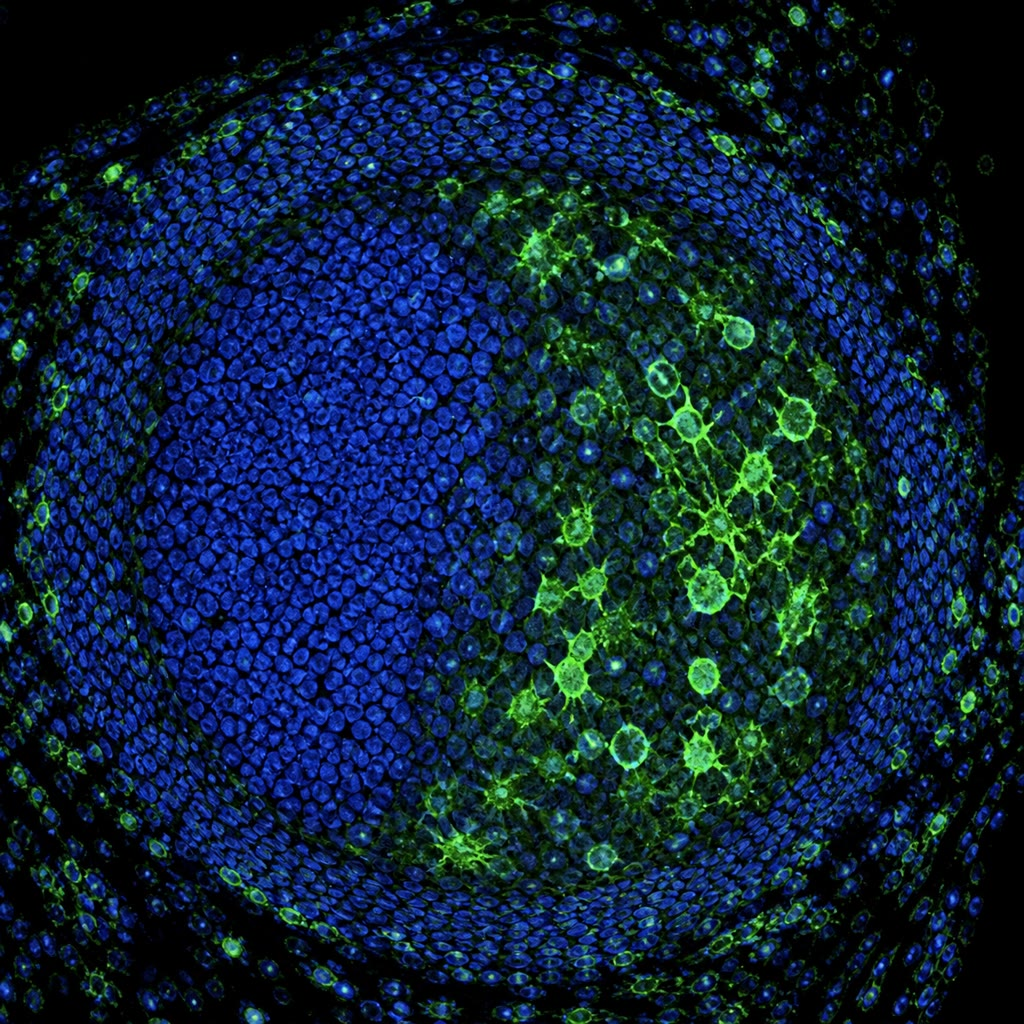
\includegraphics[width=0.36\linewidth]{images/book5/ai/b5-16-germinal-centre.jpg}\hspace{0.04\linewidth}
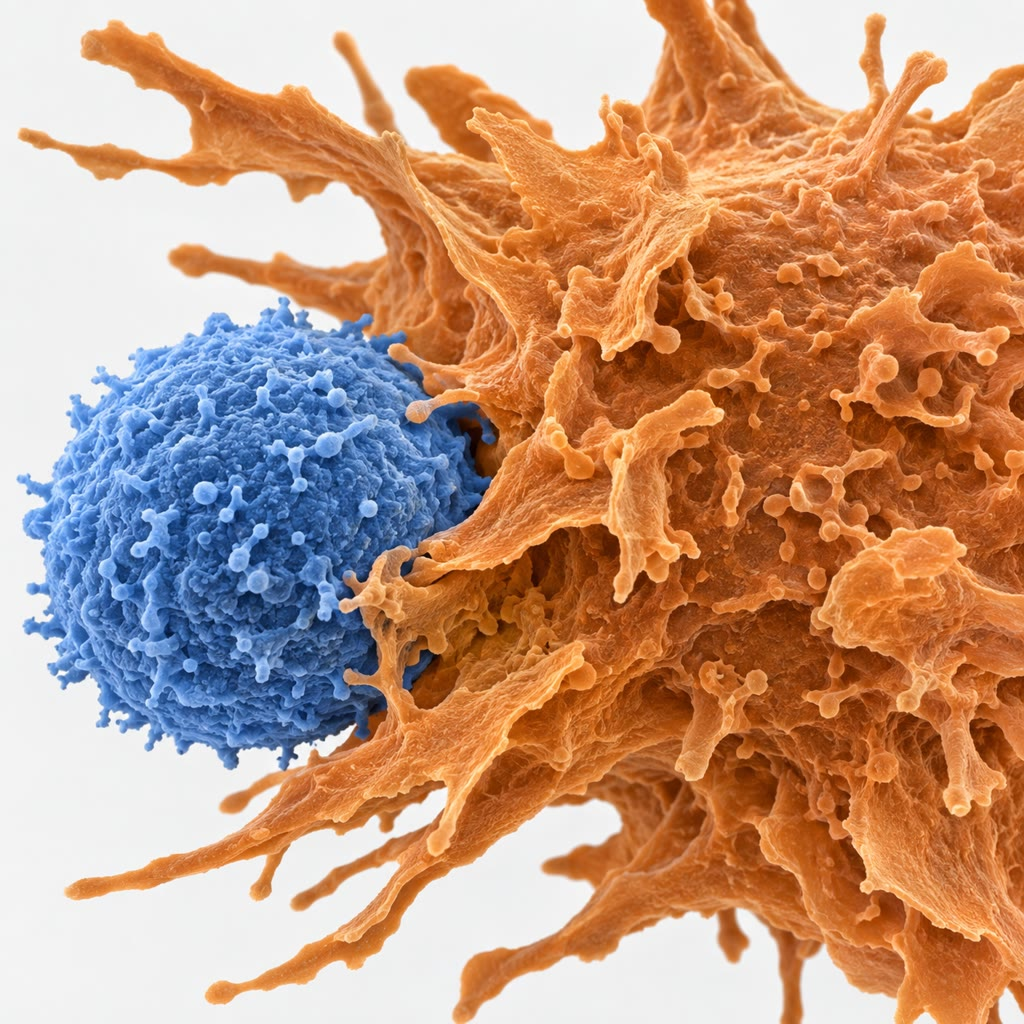
\includegraphics[width=0.36\linewidth]{images/book5/ai/b5-16-t-cell-apc.jpg}

{\small Left: a \omterm{def:b3:adaptive-immunity:germinal-centre}{germinal centre} in a \omterm{def:b3:adaptive-immunity:lymphocytes}{lymph node} --- the crowded dark
zone and the lighter zone of selection. Right: a T~cell (small) in
contact with a \omterm{def:b3:innate-immunity:innate}{dendritic cell}, the moment at which the adaptive
response is decided.}
\end{omfigure}

\section{Tolerance and its failures}

\begin{definition}[Tolerance]\label{def:b3:adaptive-immunity:tolerance}
\index{tolerance}\index{negative selection}\index{thymus}\index{anergy}\index{FoxP3}\index{autoimmunity}
The repertoire is made at random and therefore contains receptors for
self. \emph{Central tolerance} removes them where the cells mature: in
the thymus, T~cells whose receptors bind self peptide--MHC too strongly
are killed (\emph{negative selection}), those that cannot bind MHC at
all are also killed (they would be useless), and only the intermediate
few per cent leave; a transcription factor, AIRE, makes thymic cells
express proteins from every tissue --- insulin, thyroglobulin --- so
that T~cells specific for them can be deleted there. B~cells that bind
self in the marrow are deleted or edit their receptors. \emph{Peripheral
tolerance} handles the rest: a T~cell that meets its \omterm{def:b3:adaptive-immunity:lymphocytes}{antigen} without
\omterm{def:b3:adaptive-immunity:response}{costimulation} is made unresponsive (\emph{anergy}) or deleted; and
\emph{regulatory} T~cells, defined by the factor FoxP3, actively
suppress responses against self and against harmless \omterm{def:b3:adaptive-immunity:lymphocytes}{antigens} such as
food and commensals. \emph{Autoimmunity} is the failure of these
controls: type~1 diabetes (T~cells destroy the $\beta$ cells), multiple
sclerosis (myelin), rheumatoid arthritis (joints), lupus (antibodies
against nuclear components), thyroid disease; each is associated with
particular \omterm{def:b3:adaptive-immunity:mhc}{HLA} alleles, which present the relevant self peptides, and
some are triggered by infection with a microbe whose peptides resemble
a self protein (rheumatic fever after streptococcal infection).
\end{definition}

\begin{proof}[Evidence]
Medawar (1953) injected cells from one inbred mouse strain into
newborn mice of another; as adults the recipients accepted skin grafts
from the donor strain that they would otherwise have rejected, while
rejecting grafts from third strains. \omterm{def:b3:adaptive-immunity:tolerance}{Tolerance} was acquired, specific,
and set by what the immune system met early --- the experimental basis
for Burnet's deletion of self-reactive clones. Children born without a
functional AIRE gene develop \omterm{def:b3:adaptive-immunity:tolerance}{autoimmunity} against many organs at once;
those without \omterm{def:b3:adaptive-immunity:tolerance}{FoxP3} (a rare X-linked syndrome) develop fatal
\omterm{def:b3:adaptive-immunity:tolerance}{autoimmunity} in infancy --- the two arms of \omterm{def:b3:adaptive-immunity:tolerance}{tolerance}, each shown by
its absence.
\end{proof}

\begin{example}[Hypersensitivity, deficiency, transplantation]\label{ex:b3:adaptive-immunity:failures}
\emph{Allergy} is a Th2 response to a harmless \omterm{def:b3:adaptive-immunity:lymphocytes}{antigen} --- pollen,
peanut, penicillin --- that produces IgE; on re-exposure the \omterm{def:b3:adaptive-immunity:lymphocytes}{antigen}
cross-links IgE on mast cells, which release histamine within minutes,
and if the \omterm{def:b3:adaptive-immunity:lymphocytes}{antigen} is in the blood the systemic release is
\emph{anaphylaxis}, treated with adrenaline. \emph{Immunodeficiency}:
children lacking \omterm{def:b3:adaptive-immunity:antibody}{RAG} or the enzyme ADA make no \omterm{def:b3:adaptive-immunity:lymphocytes}{lymphocytes} (severe
combined immunodeficiency) and die of infection unless given marrow
or gene therapy; HIV destroys CD4 T~cells and with them the help every
response needs. \emph{Transplantation}: the recipient's T~cells see the
donor's \omterm{def:b3:adaptive-immunity:mhc}{HLA} molecules as foreign, and up to a tenth of all T~cells
respond --- far more than to any pathogen --- so grafts are matched at
the \omterm{def:b3:adaptive-immunity:mhc}{HLA} loci and the recipient is immunosuppressed for life; a graft of
marrow can attack its new host instead. And the deliberate uses: the
monoclonal antibodies of \cref{ch:b3:genetic-engineering}, the
\omterm{prop:b3:cancer-biology:immune}{checkpoint inhibitors} that release T~cells against \omterm{def:b3:cancer-biology:hallmarks}{tumours}
(\cref{ch:b3:cancer-biology}), and T~cells engineered with a chimaeric
receptor for a \omterm{def:b3:cancer-biology:hallmarks}{tumour} \omterm{def:b3:adaptive-immunity:lymphocytes}{antigen} (CAR-T), which have cured leukaemias
that nothing else touched.
\end{example}

\section{Vaccination}

\begin{definition}[Vaccines and herd immunity]\label{def:b3:adaptive-immunity:vaccine}
\index{vaccine}\index{herd immunity}\index{basic reproduction number}\index{vaccine efficacy}
A \emph{vaccine} presents \omterm{def:b3:adaptive-immunity:lymphocytes}{antigens} of a pathogen, with an adjuvant or
in a form that triggers innate receptors, so that the recipient
acquires \omterm{def:b3:adaptive-immunity:response}{memory cells} and antibodies without the disease
(\cref{ch:b3:virology} lists the kinds). Its \emph{efficacy} $E$ is the
fraction of vaccinated people protected. Protection extends beyond the
vaccinated: a pathogen spreading in a population where each case
infects $R_{0}$ others on average when all are susceptible --- the
\emph{basic reproduction number} --- infects only $R_{0}$ times the
susceptible fraction when some are immune, and dies out when that
number falls below one. This is \emph{herd immunity}: above a threshold
of immune people the chain of transmission breaks and the unvaccinated
--- infants, the immunocompromised, those in whom the vaccine failed
--- are protected by the others.
\end{definition}

\begin{theorem}[The herd immunity threshold]\label{thm:b3:adaptive-immunity:herd}
\index{herd immunity!threshold}\index{SIR model}
In a population where a fraction $p$ is immune and the rest
susceptible, each case infects on average $R_{\text{eff}} = R_{0}(1 -
p)$ others. An epidemic cannot start if $R_{\text{eff}} < 1$, that is
if
\[
p > p_{c} = 1 - \frac{1}{R_{0}} .
\]
With a \omterm{def:b3:adaptive-immunity:vaccine}{vaccine} of efficacy $E$, the coverage needed is $f_{c} = p_{c}/E$.
If an epidemic does run in a susceptible population (the \omterm{thm:b3:adaptive-immunity:herd}{SIR model},
with infection rate $\beta$ and recovery rate $\gamma$, $R_{0} =
\beta/\gamma$), it peaks when the susceptible fraction has fallen to
$1/R_{0}$, and the fraction never infected, $s_{\infty}$, satisfies
$\ln s_{\infty} = -R_{0}(1 - s_{\infty})$.
\end{theorem}
\begin{proof}
Each case makes contacts that would infect $R_{0}$ people if all were
susceptible; a fraction $1 - p$ of them are, so $R_{\text{eff}} =
R_{0}(1-p)$, and the condition $R_{\text{eff}} < 1$ gives $p_{c}$; a
\omterm{def:b3:adaptive-immunity:vaccine}{vaccine} that protects a fraction $E$ of those who receive it makes a
fraction $Ef$ of the population immune, so $Ef > p_{c}$. In the \omterm{thm:b3:adaptive-immunity:herd}{SIR
model}, $\mathrm{d}s/\mathrm{d}t = -\beta si$ and $\mathrm{d}i/\mathrm{d}t =
\beta si - \gamma i = \gamma i(R_{0}s - 1)$, so $i$ grows while $s >
1/R_{0}$ and falls after: the peak is at $s = 1/R_{0}$. Dividing the
two equations, $\mathrm{d}i/\mathrm{d}s = -1 + 1/(R_{0}s)$, so $i + s -
\ln s/R_{0}$ is constant; evaluating it at the start ($s = 1$, $i
\approx 0$) and at the end ($i = 0$, $s = s_{\infty}$) gives
$s_{\infty} - \ln s_{\infty}/R_{0} = 1$, the final-size relation.
\end{proof}

\begin{example}[Measles and smallpox]\label{ex:b3:adaptive-immunity:measles}
Measles has $R_{0} \approx 15$: $p_{c} = 1 - 1/15 = 93\,\%$, and with a
\omterm{def:b3:adaptive-immunity:vaccine}{vaccine} of efficacy $97\,\%$ after two doses the coverage needed is
$96\,\%$ --- which is why measles returns wherever vaccination slips a
few per cent, and why an unvaccinated child in a well-vaccinated
country is nonetheless safe. Smallpox had $R_{0} \approx 5$--$7$, a
threshold near $80$--$85\,\%$, no animal reservoir, no asymptomatic
carriers and a \omterm{def:b3:adaptive-immunity:vaccine}{vaccine} that worked in one dose: eradicable, and
eradicated. Polio is nearly there. Influenza and the coronaviruses,
whose \omterm{def:b3:adaptive-immunity:lymphocytes}{antigens} drift (\cref{ch:b3:virology}) and whose immunity wanes,
are not. In an unvaccinated population an epidemic with $R_{0} = 3$
infects, by the final-size relation, $1 - s_{\infty} = 94\,\%$ of
people; with $R_{0} = 1.5$, $58\,\%$.
\end{example}

\begin{omfigure}
\begin{tikzpicture}
\begin{axis}[
  width=6.4cm, height=5.4cm,
  axis x line=bottom, axis y line=left,
  xmin=1, xmax=18, ymin=0, ymax=1,
  xlabel={$R_{0}$}, ylabel={threshold $p_{c}$},
  xlabel style={font=\small, at={(axis description cs:0.5,-0.12)}, anchor=north}, ylabel style={font=\small},
  tick label style={font=\scriptsize}, xtick={1,3,6,9,12,15,18}, ytick={0,0.5,0.8,0.93,1}, yticklabels={0,0.5,0.8,0.93,1},
  clip=false,
]
\addplot[very thick, omDef, domain=1:18, samples=80] {1-1/x};
\fill[omThm] (axis cs:15,0.933) circle (2pt); \node[font=\scriptsize, anchor=south east] at (axis cs:15,0.94) {measles};
\fill[omThm] (axis cs:6,0.833) circle (2pt); \node[font=\scriptsize, anchor=north west] at (axis cs:6.3,0.82) {smallpox};
\fill[omThm] (axis cs:2.5,0.6) circle (2pt); \node[font=\scriptsize, anchor=north west] at (axis cs:2.6,0.58) {1918 influenza};
\end{axis}
\begin{axis}[
  at={(7.6cm,0)}, anchor=south west,
  width=6.4cm, height=5.4cm,
  axis x line=bottom, axis y line=left,
  xmin=0, xmax=60, ymin=0, ymax=0.35,
  xlabel={days}, ylabel={fraction infectious},
  xlabel style={font=\small, at={(axis description cs:0.5,-0.12)}, anchor=north}, ylabel style={font=\small},
  tick label style={font=\scriptsize}, xtick={0,20,40,60}, ytick={0,0.1,0.2,0.3},
  clip=false,
]
\addplot[very thick, omThm, smooth] coordinates {(0,0.001) (5,0.003) (10,0.012) (15,0.04) (20,0.12) (25,0.25) (28,0.30) (31,0.27) (35,0.18) (40,0.09) (45,0.04) (50,0.015) (55,0.006) (60,0.002)};
\addplot[very thick, omDef, smooth] coordinates {(0,0.001) (5,0.0015) (10,0.0025) (15,0.004) (20,0.006) (25,0.009) (30,0.012) (35,0.014) (40,0.015) (45,0.014) (50,0.012) (55,0.009) (60,0.007)};
\node[font=\scriptsize, omThm, anchor=west] at (axis cs:30,0.3) {no immunity, $R_{0} = 3$};
\node[font=\scriptsize, omDef, anchor=south west] at (axis cs:32,0.03) {\qty{60}{\%} vaccinated: $R_{\text{eff}} = 1.2$};
\end{axis}
\end{tikzpicture}

{\small Left: the threshold $1 - 1/R_{0}$ --- the more contagious the
disease, the closer to everyone must be immune. Right: an SIR epidemic
with $R_{0} = 3$ in a naive population and in one with \qty{60}{\%}
immune, which is not enough to stop it but flattens and slows it.}
\end{omfigure}

\begin{omfigure}
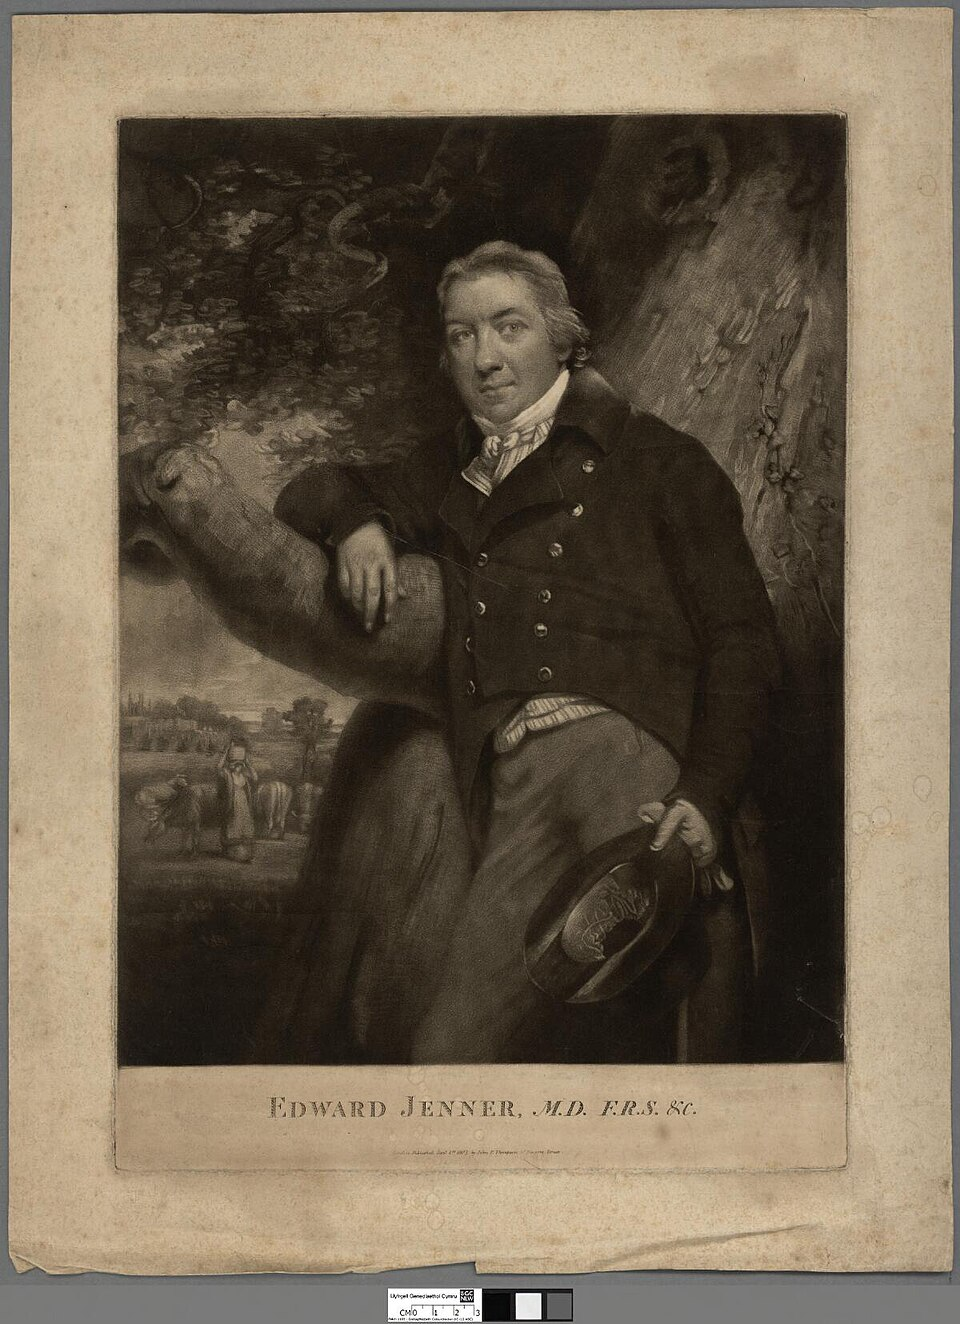
\includegraphics[width=0.30\linewidth]{images/book5/jenner.jpg}\hspace{0.04\linewidth}
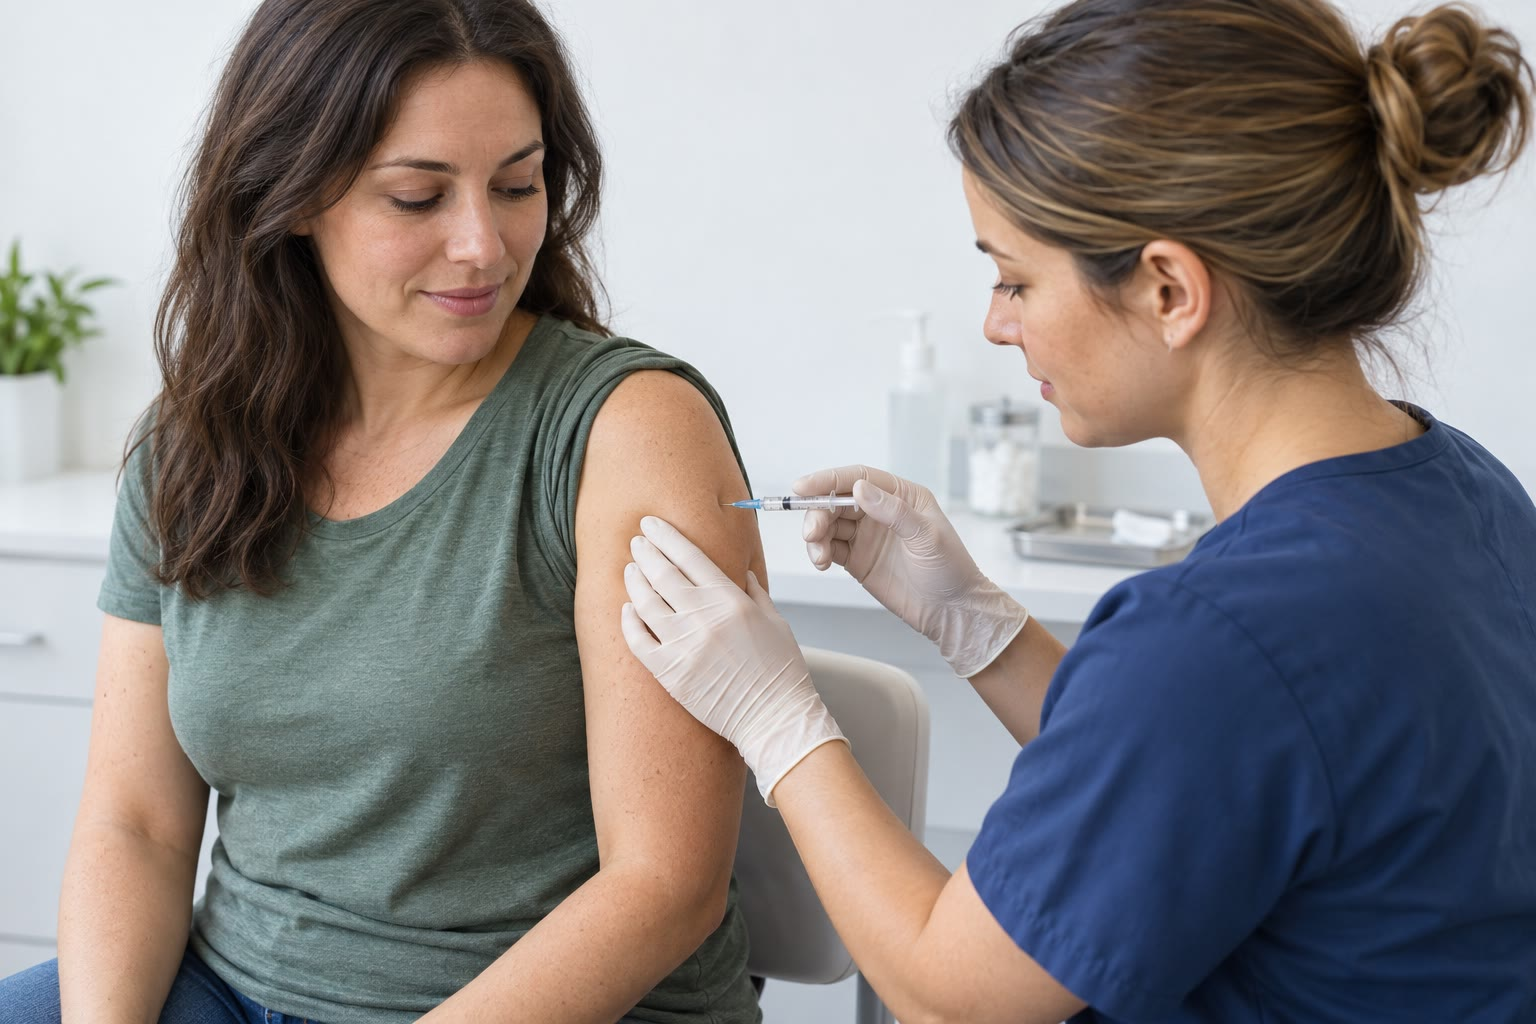
\includegraphics[width=0.50\linewidth]{images/book5/ai/b5-16-vaccination.jpg}

{\small Edward Jenner, who in 1796 protected a boy against smallpox with
cowpox and founded vaccination (engraving of 1807, public domain).
Right: the same act two centuries on --- an intramuscular \omterm{def:b3:adaptive-immunity:vaccine}{vaccine}, whose
\omterm{def:b3:adaptive-immunity:lymphocytes}{antigen} the deltoid's \omterm{def:b3:innate-immunity:innate}{dendritic cells} will carry to the axillary \omterm{def:b3:adaptive-immunity:lymphocytes}{lymph
nodes}.}
\end{omfigure}

\begin{remark}[What immunity remembers]\label{rem:b3:adaptive-immunity:memory}
The adaptive immune system is a Darwinian machine inside each of us:
random variation (V(D)J, hypermutation), selection (by \omterm{def:b3:adaptive-immunity:lymphocytes}{antigen}, in the
\omterm{def:b3:adaptive-immunity:germinal-centre}{germinal centre}, against self in the \omterm{def:b3:adaptive-immunity:tolerance}{thymus}) and inheritance (\omterm{def:b3:adaptive-immunity:response}{memory
cells}, clonal expansion). It solves, in weeks, the problem that
evolution solves in millennia --- a molecule that binds a target never
seen before --- and its answers are among the best-studied cases of
evolution observed directly. Its cost is \omterm{def:b3:adaptive-immunity:tolerance}{autoimmunity}, its dependence on
the innate system's judgement is absolute, and its memory, which
Jenner exploited and which \omterm{def:b3:adaptive-immunity:vaccine}{vaccines} write deliberately, is the reason a
species of long-lived, slow-breeding animals can survive in a world of
fast-breeding microbes.
\end{remark}

\section{Exercises}

\begin{exercise}[$\star$]\label{exo:b3:adaptive-immunity:1}
State the four tenets of \omterm{def:b3:adaptive-immunity:lymphocytes}{clonal selection} and the experiment that
supports each of the first two.
\end{exercise}

\begin{exercise}[$\star$]\label{exo:b3:adaptive-immunity:2}
Describe an \omterm{def:b3:adaptive-immunity:antibody}{antibody}'s structure and give the function of each of the
five classes.
\end{exercise}

\begin{exercise}[$\star$]\label{exo:b3:adaptive-immunity:3}
Contrast \omterm{def:b3:adaptive-immunity:mhc}{MHC class~I} and class~II in cell distribution, source of
peptide, peptide length and the T~cell that reads each.
\end{exercise}

\begin{exercise}[$\star$]\label{exo:b3:adaptive-immunity:4}
Define $R_{0}$ and the \omterm{def:b3:adaptive-immunity:vaccine}{herd immunity} threshold, and compute the
threshold for mumps ($R_{0} = 5$), pertussis ($R_{0} = 12$) and the
1918 influenza ($R_{0} = 2.5$).
\end{exercise}

\begin{exercise}[$\star\star$]\label{exo:b3:adaptive-immunity:5}
A species has $V_{H} = 50$, $D = 20$, $J_{H} = 5$ and a single light
locus with $V = 60$, $J = 4$. Compute the combinatorial repertoire, then
the total with a junctional factor of $10^{4}$. How does it compare
with the $10^{9}$ B~cells the animal has?
\end{exercise}

\begin{exercise}[$\star\star$]\label{exo:b3:adaptive-immunity:6}
A germinal-centre B~cell's variable region is \qty{1000}{bp}; AID mutates
at $10^{-3}$ per base pair per division. Over $20$ divisions, how many
mutations per cell, and among $10^{5}$ cells how many distinct
single-base variants of the \omterm{def:b3:adaptive-immunity:antibody}{antibody} are generated? Compare with the
$3000$ possible single substitutions.
\end{exercise}

\begin{exercise}[$\star\star$]\label{exo:b3:adaptive-immunity:7}
Explain why a T~cell from one person does not recognise viral peptides
presented by another person's cells, and why this same fact makes
transplants difficult and the \omterm{def:b3:adaptive-immunity:mhc}{HLA} system polymorphic.
\end{exercise}

\begin{exercise}[$\star\star$]\label{exo:b3:adaptive-immunity:8}
Predict the immune phenotype of a child lacking (a) RAG1, (b) AIRE,
(c) \omterm{def:b3:adaptive-immunity:tolerance}{FoxP3}, (d) the class-switch enzyme AID, and (e) CD4 T~cells.
\end{exercise}

\begin{exercise}[$\star\star$]\label{exo:b3:adaptive-immunity:9}
A \omterm{def:b3:adaptive-immunity:vaccine}{vaccine} has efficacy \qty{90}{\%} and the disease $R_{0} = 6$. What
coverage stops transmission? If coverage is \qty{80}{\%}, what is
$R_{\text{eff}}$, and what fraction of the population does an epidemic
infect (use the final-size relation with $R_{0}$ replaced by
$R_{\text{eff}}$ among the susceptibles --- or argue why that is
approximately right)?
\end{exercise}

\begin{exercise}[$\star\star\star$]\label{exo:b3:adaptive-immunity:10}
Derive the final-size relation of the theorem from the SIR equations
and solve it numerically for $R_{0} = 1.5$, $2$, $3$ and $5$. Why does
an epidemic never infect everyone even without any intervention?
\end{exercise}

\begin{exercise}[$\star\star\star$]\label{exo:b3:adaptive-immunity:11}
\omterm{def:b3:adaptive-immunity:germinal-centre}{Affinity maturation} raises binding a thousandfold in three weeks.
Treat the \omterm{def:b3:adaptive-immunity:germinal-centre}{germinal centre} as a population under selection: with a
mutation rate of one per cell per division, a fraction $10^{-2}$ of
mutations improving affinity by a factor $1.5$ and the rest neutral or
harmful, how many rounds of selection are needed for a thousandfold
gain, and how many cells must each round screen? Comment on why the
\omterm{def:b3:adaptive-immunity:germinal-centre}{germinal centre} is organised in cycles.
\end{exercise}

\begin{exercise}[$\star\star\star$]\label{exo:b3:adaptive-immunity:12}
Autoimmune diseases are commoner in women and associated with \omterm{def:b3:adaptive-immunity:mhc}{HLA}
alleles; type~1 diabetes has risen fivefold in fifty years in rich
countries. Propose, with the mechanisms of this chapter and of
\cref{ch:b3:microbiomes}, explanations for each observation and one
test of each.
\end{exercise}

\section{Problem: A Vaccine Campaign}

\begin{problem}[{Weekend problem --- a repertoire counted, a response
timed from a hundred cells to a millilitre of serum, a germinal centre
run as an evolutionary algorithm, and a measles campaign planned against
the herd threshold, ending on the size of the repertoire, the antibody
a plasma cell makes in a day and the coverage a country needs}]
\label{pb:b3:adaptive-immunity:1}
Data: $V_{H} = 40$, $D = 25$, $J_{H} = 6$; light loci $(40, 5)$ and
$(30, 4)$; junctional factor $3\times 10^{4}$. A body has $10^{11}$
B~cells; one in $10^{5}$ binds a given epitope; $100$ precursors are
recruited; division every \qty{8}{h} for $7$ days; \qty{30}{\%} of the
clone becomes \omterm{def:b3:adaptive-immunity:response}{plasma cells} secreting $2000$ IgG molecules a second
each; IgG is \qty{150}{kDa}; plasma volume \qty{3}{L}; IgG half-life
\qty{21}{d}. \omterm{def:b3:adaptive-immunity:germinal-centre}{Germinal centre}: \qty{1000}{bp} variable region, $10^{-3}$
mutations per bp per division, one in $100$ mutations improves
affinity by $1.5$. Measles: $R_{0} = 15$, \omterm{def:b3:adaptive-immunity:vaccine}{vaccine efficacy} $0.93$
after one dose and $0.97$ after two; a country of $5\times 10^{6}$
people with $60\,000$ births a year.

\medskip
\noindent\textbf{Part I --- The repertoire.}
\begin{enumerate}
  \item Compute the combinatorial repertoire and the total with
        \omterm{def:b3:adaptive-immunity:antibody}{junctional diversity}.
  \item Compare with the number of B~cells. What fraction of the
        possible repertoire does one body express at a time, and what
        follows for two individuals' repertoires?
  \item How many B~cells in the body bind the epitope? How many, on
        average, in a \omterm{def:b3:adaptive-immunity:lymphocytes}{lymph node} holding $10^{8}$ B~cells?
  \item A newborn has $10^{9}$ B~cells. How many bind the epitope, and
        why is a newborn's response weak even so?
  \item An \omterm{def:b3:adaptive-immunity:antibody}{antibody}'s third heavy-chain loop is made by \omterm{def:b3:adaptive-immunity:antibody}{junctional
        diversity}. Explain why this loop is the most variable part of
        the molecule and usually at the centre of the binding site.
  \item \omterm{def:b3:adaptive-immunity:germinal-centre}{Somatic hypermutation} adds diversity after selection, V(D)J
        before. Why is it advantageous to have both, in that order?
\end{enumerate}

\medskip
\noindent\textbf{Part II --- The response.}
\begin{enumerate}[resume]
  \item From $100$ cells dividing every \qty{8}{h}, how many after $7$
        days? How many \omterm{def:b3:adaptive-immunity:response}{plasma cells}?
  \item How many IgG molecules do they secrete per day, and what mass?
        What serum concentration does one day's output give in
        \qty{3}{L}?
  \item After ten days of secretion at that rate, ignoring decay, what
        is the concentration in g/L? Compare with the normal total IgG
        of \qty{10}{g/L}.
  \item The \omterm{def:b3:adaptive-immunity:response}{plasma cells} die after two weeks; the \omterm{def:b3:adaptive-immunity:antibody}{antibody} then decays
        with half-life \qty{21}{d}. How long until the concentration of
        question 9 falls a hundredfold? What maintains \omterm{def:b3:adaptive-immunity:antibody}{antibody} for
        years?
  \item A secondary response starts from $10^{5}$ \omterm{def:b3:adaptive-immunity:response}{memory cells}. How
        many cells after $3$ days, and how does that compare with the
        primary response at day 3 and day 7?
  \item Explain why IgM comes first and IgG later in a primary
        response, and why the secondary response is IgG from the start.
\end{enumerate}

\medskip
\noindent\textbf{Part III --- The \omterm{def:b3:adaptive-immunity:germinal-centre}{germinal centre}.}
\begin{enumerate}[resume]
  \item How many mutations does a B~cell acquire in its variable region
        per division? Over $20$ divisions?
  \item What fraction of the daughters of one division carry an
        improving mutation? In a \omterm{def:b3:adaptive-immunity:germinal-centre}{germinal centre} of $10^{4}$ dividing
        cells, how many improved cells appear per division?
  \item How many successive improvements of $1.5$ give a thousandfold
        gain in affinity? If each round of selection takes two
        divisions (\qty{12}{h}), how long is that?
  \item Most mutations damage the \omterm{def:b3:adaptive-immunity:antibody}{antibody}. If \qty{50}{\%} of mutations
        destroy binding, what fraction of cells survive each division's
        mutation, and why must the light zone kill most cells?
  \item A \omterm{def:b3:adaptive-immunity:vaccine}{vaccine} given as two doses six weeks apart yields antibodies
        of higher affinity than one dose. Explain with the \omterm{def:b3:adaptive-immunity:germinal-centre}{germinal
        centre}.
  \item Some viruses (HIV, influenza) escape antibodies by mutating
        their surface. Explain why the \omterm{def:b3:adaptive-immunity:germinal-centre}{germinal centre} is nevertheless
        the basis of hope for a broadly protective \omterm{def:b3:adaptive-immunity:vaccine}{vaccine}.
\end{enumerate}

\medskip
\noindent\textbf{Part IV --- The campaign.}
\begin{enumerate}[resume]
  \item Herd threshold for measles, and coverage required with one
        dose; with two doses.
  \item The country vaccinates \qty{90}{\%} of children with two doses.
        Fraction immune, $R_{\text{eff}}$, and the verdict: does measles
        circulate?
  \item How many susceptible children accumulate per year of births at
        \qty{90}{\%} coverage (unvaccinated plus \omterm{def:b3:adaptive-immunity:vaccine}{vaccine} failures)? After
        five years without measles, how many susceptibles are there,
        and why does an importation then cause an outbreak?
  \item Use the final-size relation with the effective reproduction
        number among susceptibles to estimate what fraction of those
        susceptibles an outbreak infects. (Take $R_{\text{eff}}$ from
        question 20 as the reproduction number in the whole population,
        and note that among the susceptible pool the disease spreads
        as if $R_{0}$ were $R_{\text{eff}}$.)
  \item Coverage is raised to \qty{95}{\%} with two doses. Fraction
        immune and $R_{\text{eff}}$; is the threshold met?
  \item Infants under one year cannot be vaccinated against measles
        and are the most likely to die of it. Explain how the campaign
        protects them, and what happens to their protection if coverage
        falls to \qty{85}{\%}.
  \item Summarise: the total repertoire (question~1), the IgG one day's
        \omterm{def:b3:adaptive-immunity:response}{plasma cells} make (question~8), and the two-dose coverage the
        country needs (question~19).
\end{enumerate}
\end{problem}
